\documentclass{article}
\usepackage{amssymb}
\usepackage{tikz}
\usetikzlibrary{positioning}

\begin{document}
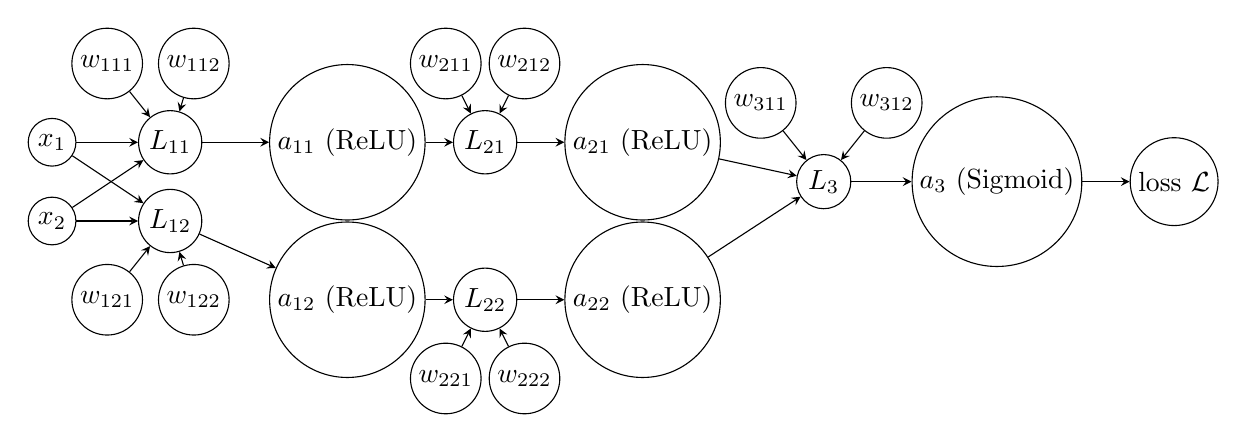
\begin{tikzpicture}[%
    activation/.style={%
        draw,
        circle,
        inner sep=2pt,
        minimum size=0.5cm,
        node distance=0.5cm
    },
    input/.style={%
        draw,
        circle,
        inner sep=2pt,
        minimum size=0.5cm,
        node distance=0.5cm
    },
    inputLayer/.style={%
        draw,
        circle,
        inner sep=2pt,
        minimum size=0.5cm,
        node distance=0.5cm
    },
    hidden/.style={%
        draw,
        circle,
        inner sep=2pt,
        minimum size=0.5cm,
        node distance=0.5cm
    },
    output/.style={%
        draw,
        circle,
        inner sep=2pt,
        minimum size=0.5cm,
        node distance=0.5cm
    },
    >=stealth
]

% Inputs
    \node[input] (input1) at (1,1) {$x_1$};
    \node[input] (input2) at (1,0) {$x_2$};

% Input layer 1 (L_1)
    \node[inputLayer] (inputLayer1) at (2.5,1) {$L_{11}$};
    \node[inputLayer] (inputLayer2) at (2.5, 0) {$L_{12}$};
    \node[inputLayer] (weight111) at (1.7, 2) {$w_{111}$};
    \node[inputLayer] (weight112) at (2.8, 2) {$w_{112}$};
    \node[inputLayer] (weight121) at (1.7, -1) {$w_{121}$};
    \node[inputLayer] (weight122) at (2.8, -1) {$w_{122}$};

% Input Layer Activation
    \node[activation] (activation11) at (4.75, 1) {$a_{11}$ (ReLU)};
    \node[activation] (activation12) at (4.75, -1) {$a_{12}$ (ReLU)};

% Hidden layer 2 (L_2)
    \node[hidden] (hidden1) at (6.5, 1) {$L_{21}$};
    \node[hidden] (hidden2) at (6.5, -1) {$L_{22}$};
    \node[hidden] (weight211) at (6, 2) {$w_{211}$};
    \node[hidden] (weight212) at (7, 2) {$w_{212}$};
    \node[hidden] (weight221) at (6, -2) {$w_{221}$};
    \node[hidden] (weight222) at (7, -2) {$w_{222}$};

%

% Hidden Layer Activation
    \node[activation] (activation21) at (8.5, 1) {$a_{21}$ (ReLU)};
    \node[activation] (activation22) at (8.5, -1) {$a_{22}$ (ReLU)};
% Output layer (L_3)
    \node[output] (output1) at (10.8, 0.5) {$L_{3}$};
    \node[output] (weight311) at (10, 1.5) {$w_{311}$};
    \node[output] (weight312) at (11.6, 1.5) {$w_{312}$};

% Output Layer activation
    \node[activation] (activation3) at (13, 0.5) {$a_{3}$ (Sigmoid)};

% Loss
    \node[output] (loss) at (15.25, 0.5) {loss $\mathcal{L}$};

% Arrows
\draw[->] (input1) -- (inputLayer1);
\draw[->] (input1) -- (inputLayer2);
\draw[->] (input2) -- (inputLayer1);
\draw[->] (input2) -- (inputLayer2);


\draw[->] (weight111) -- (inputLayer1);
\draw[->] (weight112) -- (inputLayer1);
\draw[->] (weight121) -- (inputLayer2);
\draw[->] (weight122) -- (inputLayer2);

\draw[->] (inputLayer1) -- (activation11);
\draw[->] (inputLayer2) -- (activation12);

\draw[->] (activation11) -- (hidden1);
\draw[->] (activation12) -- (hidden2);

\draw[->] (weight211) -- (hidden1);
\draw[->] (weight212) -- (hidden1);
\draw[->] (weight221) -- (hidden2);
\draw[->] (weight222) -- (hidden2);


\draw[->] (hidden1) -- (activation21);
\draw[->] (hidden2) -- (activation22);

\draw[->] (activation21) -- (output1);
\draw[->] (activation22) -- (output1);

\draw[->] (output1) -- (activation3);


\draw[->] (weight311) -- (output1);
\draw[->] (weight312) -- (output1);


\draw[->] (activation3) -- (loss);

\end{tikzpicture}

\end{document}
